
Given\begin{align}\label{ma2017-46:5}
\pr{X=n} = \begin{cases}
    \brak{\frac{1}{4}}\brak{\frac{3}{4}}^{n-1} & n=1,2 \ldots \\
    0 & otherwise
\end{cases}
\end{align}
Using the linearity of the expectation operator:
\begin{align}\label{ma2017-46:eq-1}
 E[X - 3 \mid X > 3] = E[X \mid X > 3] - 3
\end{align}
Now ,
\begin{align}
E[X \mid X > 3] &= \sum_{x=1}^{\infty} x  \pr{X=x \mid X > 3}\\
& = \sum_{x=1}^{\infty} x \frac{\pr{X=x, X > 3}}{\pr{X > 3}}\label{ma2017-46:eq1}
\end{align}
Calculating $\pr{X>3}$
\begin{align}
\pr{X > 3} =& 1 - \pr{X \leq 3}   \\
=& 1 - \sum_{x'=1}^3 \pr{X=x'} \\
=& 1 - \sum_{x'=1}^3 \brak{\frac{3}{4}}^{x'-1}\brak{\frac{1}{4}}\\
=& \frac{27}{64} \label{ma2017-46:eq2}
\end{align}
%Computing $P(X=x, X > 3)$
Also,\begin{align}\label{ma2017-46:eq3}
\pr{X=x, X > 3} = \begin{cases}
    \pr{X=x} & x > 3 \\
    0 & x \leq 3
\end{cases}
\end{align}
 %Combining the numerator and denominator
Substituting \eqref{ma2017-46:eq2} and \eqref{ma2017-46:eq3} in  \eqref{ma2017-46:eq1} we get
\begin{align}
E[X \mid X > 3] 
&= \sum_{x=1}^{3} 0 + \sum_{x=4}^{\infty} \sbrak{ x   \frac{\pr{X=x}}{\frac{27}{64}} } \\
&=\frac{64}{27} \sum_{x=4}^{\infty} \sbrak{  
x\brak{\frac{1}{4}}\brak{\frac{3}{4}}^{x-1}}\\
&=\frac{16}{27}\sum_{x=4}^{\infty} \sbrak{ x \brak{\frac{3}{4}}^{x-1}}\label{ma2017-46:sub}
\end{align}

Let
\begin{align}\label{ma2017-46:S}
S&=\sum_{x=4}^{\infty} \sbrak{ x \brak{\frac{3}{4}}^{x-1}}\
\end{align}
Multiplying (\eqref{ma2017-46:S}) with  $\frac{3}{4}$ on both sides gives
\begin{align}\label{ma2017-46:3/4S}
\frac{3}{4}S&=\sum_{x=4}^{\infty} x\frac{1}{4}\left(\frac{3}{4}\right)^{x} 
\end{align}
From \eqref{ma2017-46:3/4S} and\eqref{ma2017-46:S} 
\begin{align}
S&= 4 \brak{\frac{3}{4}}^{3}+5 \brak{\frac{3}{4}}^{4}+6 \brak{\frac{3}{4}}^{5}\ldots\\
\frac{3}{4}S&= 0\brak{\frac{3}{4}}^{3}+ 4 \brak{\frac{3}{4}}^{4}+5 \brak{\frac{3}{4}}^{5}+\ldots
\end{align}
subtracting \eqref{ma2017-46:3/4S} from \eqref{ma2017-46:S} we get
\begin{align}
\frac{S}{4}&= 4 \brak{\frac{3}{4}}^{3}+ \brak{\frac{3}{4}}^{4}+\brak{\frac{3}{4}}^{5}+\brak{\frac{3}{4}}^{6}+\ldots\\
&=4 \brak{\frac{3}{4}}^{3}+\sum_{x=4}^{\infty}   \brak{\frac{3}{4}}^{x}\\
&=\frac{189}{64}
\end{align}
Substituting vale of S in \eqref{ma2017-46:sub} we get
\begin{align}
    E[X|X>3]=7
\end{align}
Thus putting this in \eqref{ma2017-46:eq-1}
\begin{align}
    E[X-3|X>3]=4
\end{align}
\begin{figure}[h]
    \centering
    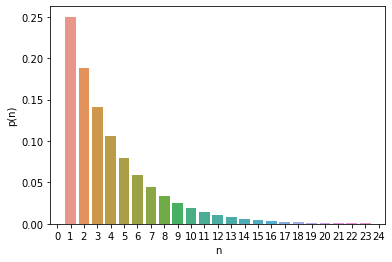
\includegraphics[width=\columnwidth]{solutions/ma/2017/46/figures/plot.png}
    \caption{PMF of $X$  }
    \label{ma2017-46:beta}
\end{figure}


